\setcounter{chapter}{ 15 }
\chapter{\textbf{Nicklepan, City Station A, Part 2} }



\subChapterTitle{``I'll Let This One Live''}


\deets{Suko}{February 20th, 2013}



We got to explode some heads, bust some jaws and bring home a trophy.  All is right with the world.  Except for all the injuries, unconsciousness, and rampant failures to follow orders.



\jumpHeadline{Nicklepan Downtown } 


\sceneHeadline{Jaya }

Jaya kicks open the roof hatch.  The armored man is only about six feet away from her and he spins around to point his rifle at her.



Jaya rushes him and tries to tackle him or at least knock him off balance.  He swings his rifle down and frees up his hands to punch her.  {[}\textit{Challenge: Duck \& Shove 2.  Matched}{]}. Jaya ducks under his swing and pushes him toward the streetside edge of the roof.



He stumbles back a step and then steps back a few more to catch his balance.  There is  an odd clicking noise like you might hear on a radio.  He says, \hl{``You should have left your VTX off.''}\footnote{\textbf{q.google }Things We Really Wish Would Be Mentioned In Her Report \#1.
Also known as ``the things the fans of the show go crazy over on the boards'' \#1. \textsubscript{03/10/13 5:49pm}}\footnote{$\rightarrow$\textbf{q.google }Though of course there's no reason she'd remember it: it's gibberish, and she's fighting for her life. \textsubscript{03/10/13 5:50pm}}  He straightens up and then starts walking forward again.



``Fuck you say!'' replies Jaya and pulls out her sidearm.  {[}\textit{Challenge: Shoot him 2.  Overcome}{]}.  



He stumbles back again and goes down to one knee.  He pulls out his sidearm and stands once again.  \hl{``Tertius, I was willing to let you go.  But now I am going to hunt down every constituent and everything related to them.  But I'll let this one live.''}\footnote{\textbf{q.google }TWRWWBMIHR \#2 \textsubscript{03/10/13 5:50pm}}\footnote{$\rightarrow$\textbf{Suko T }seconded :) \textsubscript{03/10/13 11:10pm}}  He fires at Jaya's kneecap.


\sceneHeadline{Hayley }

Meanwhile, down below, Lackovich starts putting down some cover fire and tells Hayley to run.  The other armored person starts shooting at Hayley.  {[}\textit{Challenge: Dodge sniper 2. Matched}{]}  Hayley runs as fast as she can across the street and dives gracefully through a broken window in the building that Jaya is on.  Once inside the building Hayley can hear Jaya's shouting from the roof and she races up the stairs, leaving herself entirely exposed {[}\textit{Refresh: Athletics}{]}.


\sceneHeadline{Oliver and Jonah }

Upstairs in the building that Hayley just left, Oliver has just heard Jonah cry out as he gets shot by the soldier in the back alley.  Oliver staggers over to Jonah, who is trying to staunch the bleeding but is sliding into shock.  {[}\textit{Reduce Flaw: Gunshot wound to shoulder 2 $\rightarrow$ 1}{]}.  They patch him up as best they can with their limited supplies.  Oliver is still reeling a bit from everything going on and has to devote all of his attention to helping Jonah, thus missing all of the sounds and activity going on elsewhere {[}\textit{Refresh: Focused 2}{]}.


\sceneHeadline{Jaya and Hayley }

{[}\textit{Challenge: Notice 1. Overcome}{]}. The soldier is close enough that Jaya can see that the armor is oozing some strange blue substance that is congealing.  Though she is probably more interested in the gun that is pointed at her knee.  {[}\textit{Challenge: Avoid getting kneecapped 3.  Sent back}{]}.  Because Jaya's uniform is so ill-fitting, he actually misjudges where her knee is and instead shoots her in the thigh above the knee.  {[}\textit{Challenge: Smack him in the chin.  Matched}{]} Jaya pulls out the broken chair leg she's been using as a truncheon and wallops him in the chin.  The truncheon shatters but he steps back again and draws his sidearm.



At this point Hayley bursts through the roof hatch, instantly drawing his attention.  Almost reflexively he shoots this new target.  {[}\textit{Challenge: Avoid getting shot 2.  Matched}{]}.   Hayley manages to tumble enough out of the way that the bullet gets absorbed by her armor and only leaves bruised ribs.  Jaya takes this opportunity to shoot the guy, forgetting she's just emptied her clip {[}\textit{Refresh: Sidearm 3}{]}.  While Hayley is staggering to her feet, he fires on her again \textit{{[}Challenge: Avoid getting shot, again 2.  Matched}{]} but Jaya pushes her out of the way, dislocating her own shoulder in the process. 



Over Hayley's radio, Jaya can hear Lackovich saying, ``Hayley report!''


\sceneHeadline{Jonah and Oliver }

When Hayley doesn't reply, Lackvich says over the radio, ``Constables, report!''



Woozy with pain, blood loss and shock, Jonah manages to say, ``One down, theirs.''

``Where are you?  We need to fall back.  NOW.'' orders Lackovich.

``That's going to be hard, where do we go?''

``Train tracks, the train can pick us up there.''

Jonah makes his way back across the street without getting seen.  \hl{{[}\textit{Challenge: Avoid taking stray fire or being spotted 1.  Overcome.}{]}}\footnote{\textbf{Suko T }Thanks! \textsubscript{04/06/13 4:31pm}}



Meanwhile Oliver has climbed out of the rear window and dropped to the street below, landing badly as his hands lose their grip.  {[}\textit{Refresh: Arm strength 2}{]}.  He limps over to the body of the soldier he'd shot and tries to open the helmet.  {[}\textit{Challenge: Open the helmet 2.  Matched}{]}.  Using sheer force, he rips off the faceplate to see a pale human face.  Paler than he is used to, the man is clean shaven and youngish looking.  Features are a little hard to see since the lower half of his jaw is missing, and he is definitely dead.


\sceneHeadline{Jaya and Hayley }

Jaya and Hayley exchange a look and are completely in agreement on what to do next.  They both raise their weapons and unload on the guy.  {[}\textit{Challenge: Put him down 4.  Matched}{]}.  They riddle him with holes and he stumbles back and collapses against the low wall around the edge of the roof.



Hayley rushes at him, swinging her rifle like a bat to club him in the head with it.  He says ``Sound Recall'' and pulls out a cylinder with one hand and grabs a grenade with the other.  Hayley tosses her rifle aside and instead grabs him and bodily tosses him over the edge of the roof.  Jaya can see Hayley's muscles strain painfully as she lifts him.  {[}\textit{Challenge: Toss him off the roof without going over with him 4. Matched}{]}.  As she starts lifting him over the edge, he pulls a knife and stabs her in the arm with it.  With his other hand, he smacks the cylinder against the roof edge and it collapses.  ``\hl{Initiate Glass Road}\footnote{\textbf{q.google }TWRWWBMIHR \#3 \textsubscript{03/10/13 5:56pm}}\footnote{$\rightarrow$\textbf{Suko T }Hayley remembered it, sort of.  She doesn't have an edetic memory so I had to drop some details, particularly conversational ones since she was focused on protecting Jaya.  With prompting she might remember the initiate part. \textsubscript{03/10/13 11:12pm}}`` he says as he falls.



{[}\textit{Challenge: The Glass Road.  8 Threat Tokens enter the pool}{]}



As Hayley is watching him fall, she looks up briefly, just in time to see a sniper taking aim at her.  {[}\textit{Challenge: Avoid getting shot, for the third time 2.  Sent back}{]}.  The wall Hayley was leaning on explodes and she flies backward in a shower of debris.  The impact has deafened her and left her somewhat stunned.



Jaya staggers around a little {[}\textit{Refresh: Adrenaline Junkie 2}{]} but eventually makes it over to the edge of the roof and peers over.  She can see Lackovich firing down the street at the sniper.  The sniper slings her rifle back and runs out into the street. {[}\textit{Challenge: WTF just happened? 2. Sent back}{]}  \hl{As Jaya watches in disbelief, the sniper appears to run behind an invisible wall in the middle of the street and disappears completely.}\footnote{\textbf{q.google }TWRWWBMIHR \#4 \textsubscript{03/10/13 5:57pm}}



Lackovich's voice comes over the radio getting increasingly frantic, ``Shit!  She's not at the front door.  Where did she go??  She disappeared!  Where is she?  Shitshitshit!!!!''



Jaya realizes that she has forgotten to turn her radio back on, and surreptitiously tosses her radio off somewhere so she can claim hers got lost {[}\textit{Refresh: Senior Constable 2}{]}.  Hayley sits there in a daze, unable to force herself to stand up or focus enough to do anything. {[}\textit{Refresh: Conditioned 2}{]}


\sceneHeadline{Jonah and Oliver }

Jonah uses the radio to find Oliver's position, but immediately after that, Oliver hushes his own radio.  Jonah spends some time re-adjusting and fixing his armor {[}\textit{Refresh: Armor 2}{]}. Oliver hoists the body over his shoulder and starts staggering back to where Lackovich is.  Jonah makes it to the corner where Lackovich is and can see that she seems to have a head wound and her face is covered in dirt and cement dust.  The corner that she is at has been mostly blown out, only providing partial cover.



Oliver makes it to the corner and indicates the body he's carrying, ``Got one.'' he says.

``Holy shit, is it dead?'' says Lackovich.

``Yes.''

Jonah says in astonishment, ``You grabbed the body?''

``\hl{Yeah, do you have any idea how valuable this stuff is}\footnote{\textbf{q.google }Actually yes, yes he does.

``You grabbed the body'' is not astonishment at Oliver deciding to grab it, but astonishment that Oliver \_successfully\_ grabbed it.  Jonah is \_very\_ impressed. \textsubscript{03/10/13 5:59pm}}?''replies Oliver, indicating the armor and weaponry.



``Give me your radio,'' says Lackovich and takes the radio to first try to reach Jaya. ``Fuck, she's still out there!  Come in Senior Constable, Junior Constable!''  There is no reply.



{[}\textit{Challenge: Notice 1. Overcome}{]} Oliver notices another flying machine and attempts to shoot it but his rifle gets tangled in the body the dead soldier {[}\textit{Refresh: Crack Shot 3}{]}.



Lackovich has reached Rook via the radio and he says he has locked onto our signal.  Lackovich requests an immediate evac.



Oliver tracks the flier with his rifle and is about to fire on it when Jonah tells him, ``Don't!''  Jonah says that shooting those things may be what brought all those soldiers before.  He spends some time thinking about what to do next. {[}\textit{Refresh: Small Unit Tactics 2}{]}



Oliver notices a second flier, this one on a parallel flight path some distance away. Both of them are heading away from us but are starting to loop back.



Oliver says, ``They are coming back around!  Probably coming for the train.  I will cover you while you make a break for it.''



Rook demands a report on what the things are.  

``Mechanical birds, sir.''

``Identify formation?''

``Parallel flight.  There are two, no now there are six of them.''



Oliver again encourages Lackovich and Jonah to make a break for it while he covers them, but they gang up on him and force him to come with them.  Jonah and Oliver grab the body while Lackovich leads the way to the stairs.


\sceneHeadline{Hayley and Jaya }

{[}\textit{Challenge: Notice 1. Overcome}{]} As Hayley and Jaya stumble out onto the street, Hayley looks for the body of the man she threw off the roof, but it is gone.  Jaya looks down the street and see sees a small metal object coming toward them.  {[}\textit{Challenge: Don't get blown up, again 2. Matched}{]}.  Jaya manages to push Hayley to the ground and there is a giant flash of light and a huge explosion.



Once on the ground, Jaya is unable to get back up again.  When Hayley attempts to help her to her feet, Jaya says, ``My arm's dislocated, you're going to have to pop it back in.''

Hayley looks at Jaya's shoulder consideringly and replies, ``I've had that before.  I think I know what to do.''  She takes Jaya's arm and braces herself.  ``This will probably hurt a lot, feel free to scream.''  With no more warning than that, she brutally wrenches Jaya's shoulder back into place. {[}\textit{Reduce Flaw: Dislocated left shoulder 2 $\rightarrow$ 1}{]}.  Jaya screams and passes out.



Nonplussed by this, Hayley grabs Jaya by her uniform and starts blanket-dragging her toward the stairs.  She's so focused on keeping her grip on Jaya and trying not to step on body parts that she goes straight down the middle of the road, totally exposed {[}\textit{Refresh: Athletics 2}{]}


\sceneHeadline{All together at last! }

Oliver starts shooting at the fliers to chase them off {[}\textit{Challenge: Chase off the fliers 3. Matched}{]}.  He succeeds but two of the fliers loop back and start heading toward us again. 



Jaya wakes up and sees the two fliers coming straight at them.  She yells at Hayley to move faster {[}\textit{Challenge: Get to the stairs before being divebombed 3. Sent back}{]}.  Lackovich fires at the fliers and yells, ``Get down!''



Hayley drops awkwardly to the ground and sort of falls over Jaya to partially shield Jaya's body from the blast.  There is another explosion.



Lackovich leads Oliver and Jonah down the stairs, but partway down she turns and starts heading back up.  Oliver sees her and starts to follow.

``Get on the train,'' orders Lackovich.

``No.''

``This is a Direct.  Fucking.  Order.  Get to the train!''

``Fuck you!''

Lackovich tries one last time, but gives up and runs up the stairs, with Oliver close behind.  Jonah realizes that Oliver is following Lackovich and he puts the body down and heads back up the stairs too.



{[}\textit{Challenge: Notice 1.  Overcome}{]}  Jonah realizes that the flier is arcing back again.  ``It's coming back!'' he warns.  Lackovich slings her rifle back and runs to grab Jaya.  ``Get Hayley!'' she orders Oliver and they all start running back to the stairs.



{[}\textit{Challenge: Find Shelter from the blast 3. Overcome}{]} Oliver sees the fliers getting closer and knows they won't make it to the stairs.  He shoves Hayley and Jonah toward a pile of debris and body parts and tells everyone to ``Bury yourselves!''   The blast hits and lifts them all into the air.  Oliver loses his grip on Jonah but manages to hang onto Hayley as they slam into a wall.  



Stunned but unhurt, they stagger to their feet and keep heading to the stairs.  Lackovich has dragged Jaya to the stairs and Jaya tumbles down a few steps and passes out.  Lackovich slaps her awake.



Rooks says over the radio, ``Inbound, 60 seconds.''



Hayley and Oliver make it to the stairs, with Jonah slightly behind them.  Jonah pauses to look back and sees flashes of light all throughout the city.  Hayley pauses and looks around, and gets utterly distracted by Jonah's state of dishabille.



Oliver meets Lackovich on the stairs and she tells him, ``We gotta go.''

``On it sir!'' Oliver says and picks up the body again and starts heading down the stairs.  The body is unwieldy to carry by himself and when it slips, \hl{he vents his frustration by punching it several times in the face until he calms down.}\footnote{\textbf{Suko T }Was this a refresh? \textsubscript{02/25/13 6:52pm}}



Lackovich snaps Hayley out of her daydream and yells for her and Jonah to get down to the train.



Hayley catches up to Oliver and helps him carry the body down to the train tracks.



Rook reports, ``You'll have to get on quickly, we have to get out \textit{now} or we might not be able to get out at all.''



Lackovich starts kicking down the fence next to the track and orders everyone to do the same.  The fence panel falls and we can get to the tracks just as Rook shows up with the train.



{[}\textit{Challenge: Get on board before explosion 1 (for each of us).  3 Overcome, 1 Sent back}{]}  Jaya staggers onto the train, while Hayley and Lackovich jump onboard.  Oliver is struggling with the body, and Jaya turns and snarls at him to get a move on.  Oliver gets on the train.  Jonah is the last to get on the train and the stairs behind him explode, propelling him onto the train in a cloud of dust.  The doors slide shut and the train departs.



Jaya collapses and passes out. Hayley woozily looks over at Jaya to make sure she is still breathing and then sinks to the floor in a state of \hl{semi-conciousness}\footnote{\textbf{Suko T }I'd say she was pale from massive bloodloss but there's no way you'd see it as she's probably completely covered in grey cement dust except for her right side which is caked with a mud made of dust and blood.  In retrospect, we probably should have used Street Medic here. :) \textsubscript{02/25/13 7:08pm}}.



\sceneHeadline{SAC-09} 



When the train arrives back at SAC-09, Hayley is immediately sedated and taken to MedBay.  They evaluate Jaya's condition a little longer and then sedate her too and send her to MedBay.  Jonah's shoulder is treated {[}\textit{Reduce Flaw: Gunshot wound to shoulder 1 $\rightarrow$ 0}{]}, Oliver and Lackovich are evaluated and released.



Oliver stands over the body of the soldier he shot. He doesn't want to let it out of his sight.

``We should do something with that,'' he tells Micah.

``I'm surprised you thought to bring it back.''

\hl{``They leveled Nicklepan.''}\footnote{\textbf{Suko T }I don't know who said this. \textsubscript{02/25/13 11:22pm}}\footnote{$\rightarrow$\textbf{q.google }Most likely Oliver.  There's a slight chance it was Jonah. \textsubscript{04/06/13 2:21pm}}

Oliver points at the gun that the dead soldier is carrying.  ``This gun.  Can you get me one?''

``Look kid,'' says Micah, ``you need to take a step back.''

Oliver gives Micah a hard look, ``Yeah.  I'll take ten.'' and walks off.



Jaya and Hayley spend three days in recovery in MedBay.  Oliver and Jonah are pretty much left to their own devices for a while.



That evening, Oliver is doing chinups in the bunk when there is a knock at the door.  It is Swan, looking tired, Jari and Micah.  ``You busy?'' asks Jari.  ``No,'' says Oliver.

Jari grins a little conspiratorially, ``We came to hide from KP.''  Micah holds up a bottle of liquor.  Several amenable hours pass, playing cards and drinking.



The next day, Agent Morgan stops by.  Oliver salutes her.  ``I thought I would debrief all of you together.  I wanted you to know that I'm not ignoring you.''

``Alright,'' says Oliver.

``Are you still feeling alright?''

Oliver nods and Agent Morgan leaves.

Dr. Gerhauser checks on Jaya regularly.  Jaya amuses herself trying to wheedle Swan into giving her daily sponge bath.  Hayley is a model patient of course and seems in no hurry to leave.



When Dr. Gerhauser discharges them, they get dressed and head to Ops to debrief.  Lackovich is there, as are the two Agents.



Jaya starts off the mission summary very haltingly, clearly not having prepared anything.  She reports that her team came across ``evidence'' of executions, but then grew flustered when Agent Morgan asked how she knew that.  Because she was the only one to see the bodies so clearly, none of the rest of the team could help her.  She described the bodies as two elderly women, a child and two unknowns.  All killed with a bullet to the head.



Discussion of the bodies makes Hayley turn green with nausea and she complains about the horrible smell.  



Jaya continues to describe the scene, mentioning the sudden appearance of three antagonists.  She says they were clearly antagonists because they started shooting at the squad.



At this point Lackovich jumps in and mentions the flier that Oliver shot down.  This derails the summary report as the sequence of events is sorted out.  Jonah notes that soldier seemed to appear after the flier was shot.  Oliver angrily asks if Jonah is blaming him for the soldiers appearing, which leaves Jonah non-plussed.



Jonah adds that he saw a purple flash of light before the other soldiers appeared, \hl{like one before a bomb gets dropped.}\footnote{\textbf{q.google }I didn't actually say this in session, but I forgot about the reference in the previous sessions, and Jonah wouldn't have. \textsubscript{03/10/13 6:08pm}}



When she hears this, Agent Morgan hits the intercom button and says, ``Micah, please revoke Trenton's access privileges to the evidence.''



Hayley mentions that the guy she tossed off the roof said ``sound recall''.  And later ``glass road''  Or something that sounds like that.  She also mentioned the cylinder that collapsed, and apologizes to Jaya for forgetting to grab it.  



The summary continues on for a few more minutes but is severely hampered by conflicting views of what happened and what was important.  Even the number of attackers is a little unclear.



Morgan ends the debriefing and says that everyone should write up a report for the mission and turn it in to her.



{[}\textit{\textbf{1 Token left in pool}}{]}


\sceneHeadline{Challenges \& Refreshes } 



\begin{itemize}
\item Challenge: Duck \& Shove 2.  Adrenaline Junkie 2 (Jaya) $\rightarrow$  Matched
\item Challenge: Shoot him 2.  Side arm: Empty Clip 3 (Jaya) $\rightarrow$ Overcome! \textbf{2 VP (Jaya)}
\item Challenge: Dodge sniper 2.  Athletics 2 (Hayley) $\rightarrow$ Matched
\item Refresh: Athletics (Hayley)
\item  {\color[RGB]{255,0,0}Reduce}  {\color[RGB]{255,0,0}\hl{Flaw}} \footnote{\textbf{Suko T }Because there were so freakin' many of them, I put flaws that were later reduced in session in regular un-bolded red so that you hopefully don't get repeats. \textsubscript{02/25/13 10:49pm}} {\color[RGB]{255,0,0}: Gunshot wound to shoulder 2{[}0{]} (Jonah)} .  Medkit 1 (Jonah) + Medkit 1 (Oliver) $\rightarrow$  {\color[RGB]{255,0,0}Flaw: Gunshot wound to shoulder 1{[}1{]} (Jonah)} 
\item Refresh: Focused 2 (Oliver)
\item Challenge: Notice 1. Senior Constable 2 (Jaya) $\rightarrow$ Overcome! \textbf{1 VP (Jaya)}
\item Challenge: Avoid getting kneecapped 3.  TA Uniform 1 (Jaya) + \textbf{ {\color[RGB]{255,0,0}Flaw: Wound in thigh 1{[}0{]} (Jaya)} } $\rightarrow$ Sent back
\item Challenge: Smack him in the chin 2.  Truncheon 2 (Jaya) $\rightarrow$ Matched
\item Challenge: Avoid getting shot 2.  Dancer 1 (Hayley) + \textbf{ {\color[RGB]{255,0,0}Flaw: Bruised Ribs 1{[}0{]} (Hayley)} } $\rightarrow$ Matched
\item Refresh: Sidearm 3 (Jaya)
\item Challenge: Avoid getting shot, again 2.   {\color[RGB]{255,0,0}Flaw: Dislocated left shoulder 2{[}0{]} (Jaya)}  $\rightarrow$ Matched
\item Challenge: Avoid friendly fire or being spotted 1.  Vigilant 3 (Jonah) $\rightarrow$ Overcome! \textbf{1 VP (Jonah)}
\item Refresh: Arm strength 2 (Oliver)
\item Challenge: Open the helmet 2.  Arm strength 2 (Oliver) $\rightarrow$ Matched
\item Challenge: Put him down 4.  Side Arm 3 (Jaya) + \textbf{ {\color[RGB]{255,0,0}Flaw: Wound in right arm 1{[}0{]} (Jaya)} } + Rifle 2 (Hayley) + Rifle 1 (Hayley) $\rightarrow$ Matched
\item Challenge: Toss him off the roof without going over with him 4. Athletics 2 (Hayley) + Conditioned 2 (Hayley) + Hand to Hand Combat 1 (Hayley) + TA Uniform 1 (Hayley) + \textbf{ {\color[RGB]{255,0,0}Flaw: Knife wound to upper right arm 2{[}0{]} (Hayley)} } $\rightarrow$ Matched
\item Challenge: Avoid getting shot, for the third time 2.  \textbf{ {\color[RGB]{255,0,0}Flaw: Deafened in right ear 1{[}0{]} (Hayley)} } $\rightarrow$ Sent back
\item Refresh: Adrenaline Junkie 2 (Jaya)
\item Challenge: WTF just happened? 2. \textbf{ {\color[RGB]{255,0,0}Flaw: Wait, am I tripping? 1{[}0{]} (Jaya)} } $\rightarrow$ Sent back
\item Refresh: Senior Constable 2 (Jaya)
\item Refresh: Conditioned 2 (Hayley)
\item Refresh: Armor 2 (Jonah)
\item Challenge: Notice 1. Focused 2 (Oliver) $\rightarrow$ Overcome! \textbf{1 VP (Oliver)}
\item Refresh: Crack Shot 3 (Oliver)
\item Refresh: Small Unit Tactics 2 (Jonah)
\item Challenge: Notice 1. Nose for Breadcrumbs 2 (Hayley) $\rightarrow$ Overcome! \textbf{1 VP (Hayley)}
\item Challenge: Don't get blown up, again 2. Adrenaline Junkie 2 (Jaya) $\rightarrow$ Matched
\item  {\color[RGB]{255,0,0}Reduce Flaw: Dislocated left shoulder 2{[}0{]} (Jaya)} .  Conditioned 2 (Hayley) $\rightarrow$ \textbf{ {\color[RGB]{255,0,0}Flaw: Injured shoulder 1{[}1{]} (Jaya)} }
\item Refresh: Athletics 2 (Hayley)
\item Challenge: Chase off the fliers 3. Crack shot 3 (Oliver) $\rightarrow$ Matched
\item Challenge: Get to the stairs before being dive-bombed 3. Senior Constable 2 (Jaya) $\rightarrow$ Sent back
\item Challenge: Notice 1.  Small Unit Tactics 2 (Jonah) $\rightarrow$ Overcome! \textbf{1 VP (Jonah)}
\item Challenge: Find Shelter from the blast 3. Hardened 4 (Oliver) $\rightarrow$ Overcome! \textbf{3 VP (Oliver)}
\item Challenge: Get on board before explosion 1 (for each of us).
\end{itemize}

\begin{itemize}
\item Jaya: $\rightarrow$ Sent Back
\item Hayley: Athletics 2 (Hayley) $\rightarrow$ Overcome! \textbf{1 VP (Hayley)}
\item Oliver: Grim Visage 2 (Jaya) $\rightarrow$ Overcome! \textbf{1 VP (Jaya)}
\item Jonah: Armor 2 (Jonah) $\rightarrow$ Overcome! \textbf{1 VP (Jonah)}
\end{itemize}

\begin{itemize}
\item  {\color[RGB]{255,0,0}Reduce Flaw: }  {\color[RGB]{255,0,0}Gunshot wound to shoulder}  {\color[RGB]{255,0,0} 1{[}1{]} (Jonah)} .  Street Medic 2 (Jonah) $\rightarrow$ \textbf{ {\color[RGB]{255,0,0}\hl{Quirk: Gunshot scar on shoulder}} }\footnote{\textbf{Suko T }I assume, but of course you can change it. \textsubscript{02/25/13 10:50pm}}\textbf{ {\color[RGB]{255,0,0}0{[}2{]} (Jonah)} }
\end{itemize}


\jumpHeadline{\hl{Ordinance that we lived through} }\footnote{\textbf{Suko T }Because SERIOUSLY.  DUDE.  How are they still walking? \textsubscript{02/25/13 11:10pm}}\underline{  Totals (for Sessions 15 and 16) }

Hayley: 4 occasions of people shooting at her, 5 grenades/explosions, 1 stabbing

Jaya: 4 occasions of people shooting at her, 4 grenades/explosions

Jonah: 1 occasion of people shooting at him,  3 grenades/explosions

Oliver: 3 grenades/explosions



\jumpHeadline{VP TOTALS } 

{
\parskip=0pt
Hayley: 2

Jaya: 4

Jonah: 3

Oliver: 4
}


\jumpHeadline{ Quotes } 



``Making the wound sexy makes the challenge higher so be careful''

\extraIndent{- Ion to Rebecca, discussing proposed use of Grim Visage (I think)}



``Great!  I throw my gun at him!  I mean, not literally, but the bullets in it.''

\extraIndent{ - Rebecca, fighting an armored soldier}


\quotedDialog{
``I believe in you!  That's worth nothing, but ....''

``Spoken like a leader.''
}
\extraIndent{- Rebecca (to Hayley) and Adam}



``Cool: I get a knife!''

\extraIndent{                                - Suko, after Hayley was stabbed in the arm}


\quotedDialog{
``Once again, face down in a dead body.''

``Don't lick it.''
}
\extraIndent{-Rebecca and Adam (I think?)}


\quotedDialog{
``It's a level 3 challenge to be bathed by Swan.''

``Can I hit him with my truncheon?''

``I'd hit that with a truncheon!''
}
\extraIndent{- Ion, Rebecca, Adam}




\vspace{\fill}

\begin{flushright}
\textsubscript{last edited by \textbf{Suko T} @ 06/19/15 4:21pm}
% Exported @ 08/23/15 11:58pm
\end{flushright}


\begin{flushright}
~
\vskip 30em
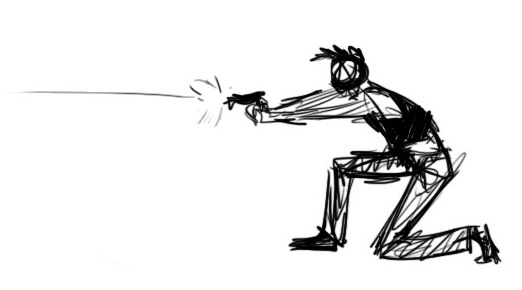
\includegraphics[width=12cm]{img/boo1_shooting_misc.jpg}
\end{flushright}
